\documentclass[titlepage]{jarticle}
\usepackage[dvipdfmx]{graphicx}
\usepackage{listings}
\usepackage{here}
\usepackage{amsmath}

%
\lstset{
  basicstyle={\ttfamily},
  identifierstyle={\small},
  % commentstyle={\smallitshape},
  keywordstyle={\small\bfseries},
  ndkeywordstyle={\small},
  stringstyle={\small\ttfamily},
  frame={tb},
  breaklines=true,
  columns=[l]{fullflexible},
  numbers=left,
  xrightmargin=0zw,
  xleftmargin=3zw,
  numberstyle={\scriptsize},
  stepnumber=1,
  numbersep=1zw,
  lineskip=-0.5ex,
  language=c
}
\renewcommand{\lstlistingname}{ソースコード}
\makeatletter
\newcommand{\figcaption}[1]{\def\@captype{figure}\caption{#1}}
\newcommand{\tblcaption}[1]{\def\@captype{table}\caption{#1}}
\makeatother
\begin{document}
\section{目的}
Gameプログラムの開発を通して、オブジェクト指向プログラミングに関する技術を習得する。
\section{システムの概要}
%・新キャラクタの動作をわかりやすく記述してください。
私が作成した新キャラクターは隠しブロックで,最初は現れておらず,隠しブロックがある場所をPlayerが下から衝突することで出現する.
出現時,Playerは隠しブロックより上に行くことはせず,速度を失う.
また,出現時は図\ref{newCharacter}のような姿をしている.
\begin{figure}[H]
  \centering
  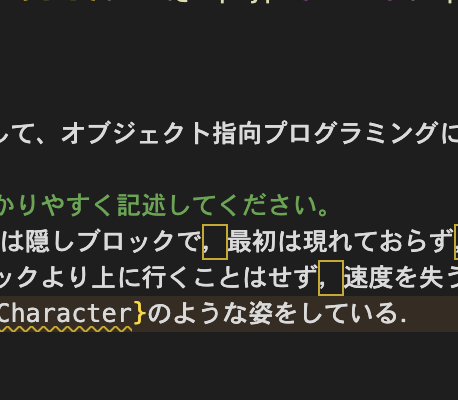
\includegraphics[width=6cm]{img/newCharacter.png}
  \caption{新キャラクター出現時の}
  \label{newCharacter}
\end{figure}
\section{システムの構成}
% ・新キャラクタ、および新キャラクタと関連を持つキャラクタをクラス図で示し、
% 新キャラクタの属性、メソッド、および他のキャラクタとの関係を
% わかりやすく説明してください。
\section{考察}
% ・今回のGame プログラム作成を踏まえて、以下を記述してください。
% ①オブジェクト指向プログラミングの長所
% ②オブジェクト指向プログラミングで注意すべき点
\section{感想}
% ※ここは採点の対象外です。
% 今回の実験の内容について感想などあれば記述して下さい。
% 次年度以降の実験の実施に役立てたいと思います。
\end{document}